%!TEX TS-program = pdflatex
%!TEX root = tesi.tex
%!TEX encoding = UTF-8 Unicode

\chapter{Basic tools}

In this chapter we introduce some notion of similarity already existing in literature and then extending them to define similarity among subgraphs in labeled graphs. 

In the last sections we present two different techniques we will use afterwards to estimate such similarity.

%%%%%%%%%%%%%%%%%%%%%%%%%%%%%%%%%%%%%%%%%%%%%%%%%%%%%%%%%%%%%%%%%%%%%%%%
%%%%%%%%%%%%%%%%%%%%%%%%%%%%%%%%%%%%%%%%%%%%%%%%%%%%%%%%%%%%%%%%%%%%%%%%
\section{Similarity indices}

\begin{definizione}\label{def:jaccard}
    Given two set $A$ and $B$ we define the \textbf{Jaccard index} as the size of the intersection divided by the size of the union between the two sets:
    
    \begin{equation}
    J(A,B) = \frac{|A \cap B|}{|A \cup B|}
    \end{equation}
    
\end{definizione}

\begin{definizione}\label{def:bray}
    Given two set $A$ and $B$ we define the \textbf{Bray-Curtis index} as:
    
    \begin{equation}
    BC(A,B) = \frac{2 \times |A \cap B|}{|A| + |B|}
    \end{equation}
    
\end{definizione}

\begin{esempio}
	Given $A = \{1, 3, 4, 5, 7, 8\}$ and $B = \{1, 2, 4, 6, 8\}$ we have:
	
	\begin{equation}
	J(A,B) = \frac{|\{1, 4, 8\}|}{|\{1, 2, 3, 4, 5, 6, 7, 8\}|} = \frac{3}{8} 
	\end{equation}
	
	\begin{equation}
	BC(A,B) = \frac{2 \times |\{1, 4, 8\}|}{|\{1, 3, 4, 5, 7, 8\}| + |\{1, 2, 4, 6, 8\}|} = \frac{6}{11} 
	\end{equation}
\end{esempio}


Note that when $A = B$ we have $J(A,B) = BC(A,B) = 1$ and when $A \cap B = \emptyset$ we have $J(A,B) = BC(A,B) = 0$.

Using set may be limiting as we consider only once the repeated values, we can easily extended the two previous definition to multiset.\\

\begin{definizione}
	A multiset is a generalization of set that allows multiple instances of elements.
\end{definizione}

To avoid confusion afterwards we use square brackets $[\ ]$ to indicate multiset and curly brackets $\{\ \}$ to indicate set.\\

Multiset can also be seen as an array of frequencies of its object (e.g. we indicate with $A = (2, 0, 3)$ the multiset with $2$ elements of first type, $0$ elements of second type and $3$ elements of third type, this notation is equivalent to write $A = [1, 1, 3, 3, 3]$).\\

 Given two multiset $A = (a_{1}, \ldots, a_{n}) $ and $B = (b_{1}, \ldots, b_{n})$ we define the following operations:

\begin{itemize}
  \item intersection $C = A \cap B  = (c_{1}, \ldots, c_{n})$ where $c_{i} = \min(a_{i}, b_{i})$
  \item union $C = A \cup B  = (c_{1}, \ldots, c_{n})$ where $c_{i} = \max(a_{i}, b_{i})$
  \item multiset union $C = A \uplus B  = (c_{1}, \ldots, c_{n})$ where $c_{i} = a_{i} + b_{i}$
\end{itemize}

\begin{definizione}\label{def:wjaccard}
    Given two multiset $A = (a_{1}, \ldots, a_{n}) $ and $B = (b_{1}, \ldots, b_{n})$ we define the \textbf{Frequency Jaccard index} as:
    
    \begin{equation}
    FJ(A,B) = \frac{\sum\limits_{i=1}^n { min(a_{i}, b_{i}) } }{\sum\limits_{i=1}^n { max(a_{i}, b_{i}) }}
    \end{equation}
    
\end{definizione}


\begin{definizione}\label{def:wbray}
    Given two multiset $A = (a_{1}, \ldots, a_{n}) $ and $B = (b_{1}, \ldots, b_{n})$ we define the \textbf{Bray-Curtis index on multiset} as:
    
    \begin{equation}
    BC(A,B) = \frac{ 2 \times \sum\limits_{i=1}^n { min(a_{i}, b_{i}) } }{\sum\limits_{i=1}^n {a_{i} + b_{i}}}
    \end{equation}
    
\end{definizione}

As a side note, Bray-Curtis is a relevant index for multisets, and is also known as Steinhaus similarity, Pielou's Similarity, Sorensen's quantitative, and Czekanowski's similarity.

\begin{esempio}
	Given $A = (0, 2, 3, 1, 0, 3) $ and $B = (2, 0, 1, 3, 1, 2)$ we have:
	
	\begin{equation}
	J(A,B) = \frac{0 + 0 + 1 + 1 + 0 + 2}{2 + 2 + 3 + 3 + 1 + 2} = \frac{4}{13} 
	\end{equation}
	
	\begin{equation}
	BC(A,B) = \frac{2 \times (0 + 0 + 1 + 1 + 0 + 2) }{2 + 2 + 4 + 4 + 1 + 4} = \frac{8}{17}
	\end{equation}
\end{esempio}


Both indices are widely used in practical application, Bray-Curtis index gives a greater weight to the intersection, on the other side the Jaccard Index is a distance metric and may be preferred to Bray-Curtis index since it is only a semi-metric distance (as it does not satisfy the triangle inequality). 

\clearpage

%%%%%%%%%%%%%%%%%%%%%%%%%%%%%%%%%%%%%%%%%%%%%%%%%%%%%%%%%%%%%%%%%%%%%%%%
%%%%%%%%%%%%%%%%%%%%%%%%%%%%%%%%%%%%%%%%%%%%%%%%%%%%%%%%%%%%%%%%%%%%%%%%
\section{Documents similarity}

Documents similarity is an hot topic in Information Retrieval, as it can be seen as the problem of duplicate detection or, from another point of view, plagiarism detection.\\

To define documents similarity we need the notion of \textit{$q$-gram}:

\begin{definizione}
	A $q$-gram is a contiguous subsequence of $q$ items from a sequence.
\end{definizione}

In this case the sequence is a document and the items can be words, characters or even syllables. If the elements used are words, $q$-gram may also be called shingles.

\begin{esempio}
	Given the document \textit{"I live and study in Pisa"} all the possible $3$-grams are: 
	\textit{"I live and"}, \textit{"live and study"}, \textit{"and study in"} and \textit{"study in Pisa"}.
\end{esempio}

Note that in a document with $n$ words the possible $q$-grams are exactly $n-q+1$.\\

It is easy to see if we use the set, or multiset, of the all possible $q$-grams of two documents we can use it to calculate their similarity based on the Jaccard or Bray-Curtis index.\\

Considering that the number of $q$-grams in a document is linear in its number of words, documents similarity is not an hard problem as we have only to perform union and intersection between set, or multiset.

\begin{esempio}
	Given the documents 
	\begin{equation*}
	A = \textit{I live, work and study in Pisa}
	\end{equation*}
	\begin{equation*}
	B = \textit{You work and study in Livorno}
	\end{equation*}
	The set of their $2$-grams are:
	\begin{equation*}
	S_{A} = (\textit{I live}, \textit{live work}, \textit{work and}, \textit{and study}, \textit{study in}, \textit{in Pisa})
	\end{equation*}
	\begin{equation*}
	S_{B} = (\textit{You work}, \textit{work and}, \textit{and study}, \textit{study in}, \textit{in Livorno})
	\end{equation*}
	The similarity using both Jaccard and Bray-Curtis are:\\
	\begin{equation*}
		J(S_{A},S_{B}) = \frac{|S_{A} \cap S_{B} |}{|S_{A} \cup S_{B} |} = \frac{3}{8}
	\end{equation*}
	\begin{equation*}
		BC(S_{A},S_{B}) = \frac{2 \times |S_{A} \cap S_{B} |}{|S_{A}| +|S_{B}|} = \frac{6}{11}
	\end{equation*}
\end{esempio}

\clearpage
%%%%%%%%%%%%%%%%%%%%%%%%%%%%%%%%%%%%%%%%%%%%%%%%%%%%%%%%%%%%%%%%%%%%%%%%
%%%%%%%%%%%%%%%%%%%%%%%%%%%%%%%%%%%%%%%%%%%%%%%%%%%%%%%%%%%%%%%%%%%%%%%%
\section{Graphs similarity}

The definition of similarity between graphs is more complex, as we have to introduce the concept of graph isomorphism.

\begin{definizione}
	An isomorphism between two graphs $G=(V_{G}, E_{G})$ and $H=(V_{H}, E_{H})$ is a bijective function from vertices of $G$ to vertices of $H$ that preserve the edge structure, i.e.  $f : V_{G} \rightarrow V_{H}$ s.t. $(v, u) \in E_{G} \implies (f(v), f(u)) \in E_{H}$.
\end{definizione}

If such isomorphism exists, the graphs are called isomorphic and we denote it with $G \simeq H$. 

\begin{esempio}
	\begin{figure}[h]
		\centering
		\begin{minipage}[t]{.45\textwidth}
			\centering
			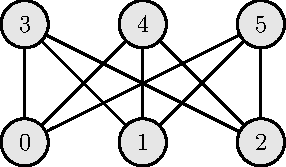
\includegraphics[width=5cm,height=3.33cm]{figure/figure-2-3}
			\caption{Graph $G$}
		\end{minipage}\hfill
		\begin{minipage}[t]{.45\textwidth}
			\centering
			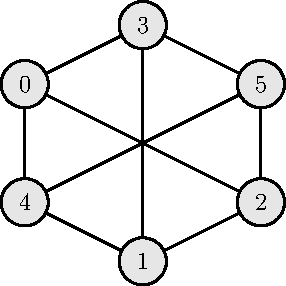
\includegraphics[width=4cm,height=4cm]{figure/figure-2-4}
			\caption{Graph $H$}
		\end{minipage}
	\end{figure}

	The two graphs are isomorphic with the function $f : V_{G} \rightarrow V_{H}$ s.t. $f(0) = 0$, $f(1) = 1$, $f(2) = 2$, $f(3) = 3$, $f(4) = 4$ and $f(5) = 5$. 
	
\end{esempio}

With the notion of graph similarity we can define a similarity between graph:

\begin{definizione}
	The similarity between two graphs $G=(V_{G}, E_{G})$ and $H=(V_{H}, E_{H})$ is the size of the largest graph isomorphism between a subgraph $G' \subseteq G$ and a subgraph $H' \subseteq H$ (seen as number of vertex of $G'$).
\end{definizione}

Unfortunately the subgraph isomorphism is a NP-complete problem, so the only way to solve it is by using methods

\clearpage
%%%%%%%%%%%%%%%%%%%%%%%%%%%%%%%%%%%%%%%%%%%%%%%%%%%%%%%%%%%%%%%%%%%%%%%%
%%%%%%%%%%%%%%%%%%%%%%%%%%%%%%%%%%%%%%%%%%%%%%%%%%%%%%%%%%%%%%%%%%%%%%%%
\section{Subgraphs similarity}

After discussing the already existing notions of similarity, we are ready to extend them to define similarity in a labeled complex network.\\

Consider a labeled graph $G = (V, E, L)$ over an alphabet $\Sigma$ where $L \rightarrow \Sigma$ is the node labeling, so that each node $u \in V$ has a label $L(u) \in \Sigma$\footnote{Alternatively we can labeling edges in $E$ instead of nodes in $V$ without making too many changes in the following definitions, for sake of simplicity we consider the graph labeled on its nodes.}, we are interest in analyzing $G$ using the sequence of labels in its path.\\

For a fixed integer $q > 0$, consider an arbitrary simple path $\pi = u_{1}, \ldots, u_{q}$, we call the orientation $u_{1} \rightarrow \ldots \rightarrow u_{q}$ of $\pi$ a $q$-path leading to $u_{q}$ and $L(\pi) = L(u_{i}) \ldots L(u_{q}) \in \Sigma^{q}$ its $q$-gram, obtained by concatenating the labels of its nodes.\footnote{Note that in an undirected graph we have, for a single simple path, two possible $q$-path, one for each orientation: one leading to $u_{q}$ from $u_{1}$ and one leading to $u_{1}$ from $u_{q}$.}.\\

For a set of nodes $A \subseteq V$, we define $L(A)$ as the corresponding multiset of $q$-grams for all $q$-path $\pi$ leading to a node $u \in A$. 
\begin{equation}
L(A) = [x \in \Sigma^{q} : \exists \text{ $q$-path } \pi \text{ leading to } u \in A \text{ with } L(\pi) = x]
\end{equation}

In this way, for each $q$-path $\pi = u_{1}, \ldots, u_{q}$ leading to $u_{q} \in A$, we have that $u_{i} \in A \cup N^{<q}(A)$ $\forall$ $1 \leq i < q$. \\

This is a good definition because, as it was mentioned before, we take into account both the internal structure of $A$ and its neighborhood $N^{<q}(A)$. 

Note that we explicitly exclude all the $q$-path both beginning and starting outside $A$, as we not considering them influential to define the similarity.\\

Given a single $q$-gram $x$ we are interested in its frequency within the multiset $L(A)$ so we define:
\begin{equation}
	f_{A}[x] = |\{ \pi : \pi \text{ is a $q$-path leading to } u \in A \text{ and } L(\pi) = x \}|
\end{equation}

With the property that $f_{A}[x] = \sum_{u \in A}{f_{\{u\}}[x]}$.

\begin{definizione}
	Given an undirected labeled graph $G = (V,E,L)$ over an alphabet $\Sigma$ and an integer $q > 0$, the Bray-Curtis similarity index between two set of nodes $A, B \subset V$ is:
	\begin{equation}	
		BC(A,B) = \frac{ 2 \times \Sigma_{x \in \Sigma^{q}} \min(f_{A}[x], f_{B}[x]) }{ \Sigma_{x \in \Sigma^{q}} f_{A}[x] + f_{B}[x] }
	\end{equation}
\end{definizione}

\begin{definizione}
	Given an undirected labeled graph $G = (V,E,L)$ over an alphabet $\Sigma$ and an integer $q > 0$, the Jaccard similarity index between two set of nodes $A, B \subset V$ is:
	\begin{equation}	
	FJ(A,B) = \frac{ \Sigma_{x \in \Sigma^{q}} \min(f_{A}[x], f_{B}[x]) }{ \Sigma_{x \in \Sigma^{q}} f_{A \cup B}[x] }
	\end{equation}
\end{definizione}

Let $\mathcal{L} = \{ x \in \Sigma^{q} : x \in L(V) \} \subseteq \Sigma^{q}$ be the set of all distinct $q$-grams found in the $q$-paths of G. Note that ranging $x$ over $\mathcal{L}$, instead of $\Sigma^{q}$, is sufficient in both the above formulas for any $A$ and $B$.\\

In general $BC(A,B) \geq FJ(A,B)$. When $A \cap B = \emptyset$ we have that $f_{A \cup B}[x] = f_{A}[x] + f_{B}[x]$ and $BC(A,B) = 2 \times FJ(A,B)$\\

% Note that given two multiset $A = (a_{1}, \ldots, a_{n}) $ and $B = (b_{1}, \ldots, b_{n})$ we define the following operations:

% \begin{itemize}
% 	\item multiset intersection $C = A \cap B  = (c_{1}, \ldots, c_{n})$ where $c_{i} = \min(a_{i}, b_{i})$
% 	\item multiset union $C = A \cup B  = (c_{1}, \ldots, c_{n})$ where $c_{i} = \max(a_{i}, b_{i})$
% 	\item multiset sum $C = A \uplus B  = (c_{1}, \ldots, c_{n})$ where $c_{i} = a_{i} + b_{i}$
% \end{itemize}

Now we present a little example to better understand.


% \begin{figure}[h]
% % 	\centering
% 	\begin{minipage}[t]{.45\textwidth}
% 		\centering
% 		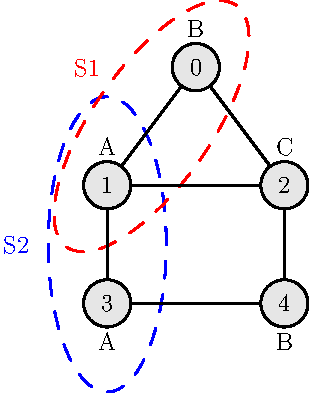
\includegraphics[width=3.9cm,height=5cm]{figure/figure-2-1}
% 	%	\caption{Labeled graph}
% 	\end{minipage}\hfill
% \end{figure}

\begin{esempio}
	We want to calculate the similarity between the two set $S_{1} = \{0,1\}$ and $S_{2} = \{1, 3\}$ using their $3$-grams of this graph:
		
	
	\begin{minipage}[t]{1\textwidth}
	\centering
	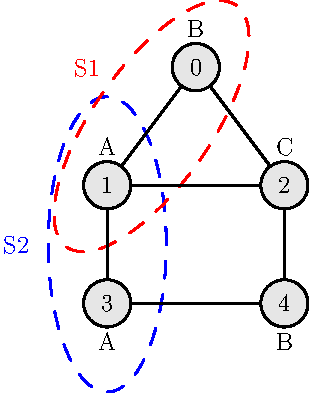
\includegraphics[width=3.9cm,height=5cm]{figure/figure-2-1}
	%	\caption{Labeled graph}
	\end{minipage}\hfill

	\begin{equation*}
		L(S_{1}) = [aab, acb, baa, bca, bca, bcb, cab, cba]
	\end{equation*}
	\begin{equation*}
		L(S_{2}) = [baa, baa, bca, bca, caa, cba, cba]
	\end{equation*}
	
	% Their union and intersection:
	
	% \begin{equation*}
	% L(S_{1}) \cup L(S_{2}) = [aab, acb, baa, bca, bca, bcb, cab, cba]
	% \end{equation*}
	% \begin{equation*}
	% L(S_{1}) \cap L(S_{2}) = [baa, baa, bca, bca, caa, cba, cba]
	% \end{equation*}
		
	So we have that:
	
	\begin{equation*}
		FJ(S_{1}, S_{2}) = \frac{4}{11} \text{  and  } BC(S_{1}, S_{2}) = \frac{8}{15}
	\end{equation*}
	
\end{esempio}

\clearpage

%%%%%%%%%%%%%%%%%%%%%%%%%%%%%%%%%%%%%%%%%%%%%%%%%%%%%%%%%%%%%%%%%%%%%%%%
%%%%%%%%%%%%%%%%%%%%%%%%%%%%%%%%%%%%%%%%%%%%%%%%%%%%%%%%%%%%%%%%%%%%%%%%
\section{Sketches}

TODO 
% \clearpage

%%%%%%%%%%%%%%%%%%%%%%%%%%%%%%%%%%%%%%%%%%%%%%%%%%%%%%%%%%%%%%%%%%%%%%%%
%%%%%%%%%%%%%%%%%%%%%%%%%%%%%%%%%%%%%%%%%%%%%%%%%%%%%%%%%%%%%%%%%%%%%%%%
\subsection*{Min-wise permutation}

TODO 
% \clearpage

%%%%%%%%%%%%%%%%%%%%%%%%%%%%%%%%%%%%%%%%%%%%%%%%%%%%%%%%%%%%%%%%%%%%%%%%
%%%%%%%%%%%%%%%%%%%%%%%%%%%%%%%%%%%%%%%%%%%%%%%%%%%%%%%%%%%%%%%%%%%%%%%%
\subsection*{Bottom-k sketches}

TODO 


%%%%%%%%%%%%%%%%%%%%%%%%%%%%%%%%%%%%%%%%%%%%%%%%%%%%%%%%%%%%%%%%%%%%%%%%
%%%%%%%%%%%%%%%%%%%%%%%%%%%%%%%%%%%%%%%%%%%%%%%%%%%%%%%%%%%%%%%%%%%%%%%%
\section{Color Coding}

TODO 
% \cite{Alon:1995:COL:210332.210337}

\clearpage
